\documentclass[conference]{IEEEtran}
\usepackage{cite}
\usepackage{graphicx}
\usepackage{amsmath,amssymb}
\usepackage{algorithmic}
\usepackage{textcomp}
\usepackage{xcolor}
\usepackage{hyperref}

\graphicspath{{./images}}

\title{Efficient Big Data Processing for Fare Estimation in Urban Transportation: A Case Study with NYC TLC Data}

\author{
  \IEEEauthorblockN{
    Youssef Ehab Abbas\IEEEauthorrefmark{1}, Youssef Fathy\IEEEauthorrefmark{2}, Hamdy Tamer Hamdy\IEEEauthorrefmark{3},\\
    Ahmed Fateen\IEEEauthorrefmark{4}, Omar Mahmoud\IEEEauthorrefmark{5}, Mohamed Hassan Ahmed\IEEEauthorrefmark{6}
  }
  \IEEEauthorblockA{
    \IEEEauthorrefmark{1}221000189, \IEEEauthorrefmark{2}221000056, \IEEEauthorrefmark{3}221001680,\\
    \IEEEauthorrefmark{4}221000093, \IEEEauthorrefmark{5}221000495, \IEEEauthorrefmark{6}221001705
  }
}

\begin{document}

\maketitle

\begin{abstract}
The rapid growth of urban transportation has led to an increasing demand for accurate and transparent taxi fare estimation. In New York City, the Taxi and Limousine Commission (TLC) provides a comprehensive dataset of yellow taxi trips spanning 2022–2023 [1], to account for seasonal demand fluctuations and post-pandemic travel behaviour shifts. This dataset includes millions of records with granular details such as GPS coordinates, timestamps, trip distances, and fare structures, enabling the identification of hidden patterns in fare determinants. By leveraging machine learning models trained on this consolidated dataset, this project aims to provide a data-driven framework for fare prediction that transcends traditional rule-based approaches, offering real-time adaptability to dynamic urban conditions like traffic congestion and event-driven demand surges.
\end{abstract}

\section{Introduction}
The NYC TLC provides a comprehensive dataset including GPS, timestamps, and fare information. Our model uses this rich dataset to offer real-time fare prediction that adapts to dynamic conditions such as traffic and demand surges.

\section{Problem Statement}
Traditional fare estimation methods often rely on simplified distance-based rules, failing to address critical variables such as temporal demand fluctuations, traffic congestion patterns, and geospatial dependencies. By utilizing [1], this project addresses these limitations through machine learning models capable of disentangling complex feature interactions. The merged dataset's expanded temporal scope ensures the model accounts for post-pandemic travel behaviour shifts and seasonal fare variations, ultimately improving prediction robustness compared to single-year analyses.

\section{Related Work}
Several studies have leveraged the NYC Taxi and Limousine Commission (TLC) dataset to explore fare prediction, trip time estimation, and operational optimization using machine learning techniques.

\subsection{Spatial Data Cleaning and Feature Engineering}
Effective data preprocessing is crucial for building accurate taxi fare prediction models. Huang [11] addressed data inconsistencies such as negative fares and exaggerated distances by implementing four data cleaning criteria, including the use of the Haversine formula to calculate distances from latitude and longitude coordinates. Similarly, Zubaid [12] emphasized the importance of handling missing values and outliers, as well as feature engineering techniques like extracting temporal features (e.g., hour, day, month) from pickup datetime fields. In another study, Ikeorah [9] integrated external datasets, including weather conditions and holiday schedules, to enhance the feature set, highlighting the significance of incorporating external factors in preprocessing steps.

Additionally, Rhouas and El Hami [10] processed over 12 million records from the NYC yellow taxi dataset, utilizing Apache Spark and Hadoop Distributed File System (HDFS) to manage and preprocess data stored in Parquet format. Their preprocessing steps included rigorous data cleaning, temporal feature extraction, and correlation analysis to identify key features influencing fare amounts, such as passenger count, trip distance, and tip amount.

A critical study by Stoyanovich et al. (CEUR-WS, Vol-2247) developed a multi-resolution preprocessing pipeline that handles the dataset's inherent spatial complexities[13]. Their methodology implemented geographic resolution layers at 10-meter, 100-meter, and 1000-meter granularity, enabling hierarchical analysis of trip patterns. The preprocessing workflow included coordinate normalization using Web Mercator projection (EPSG:3857) and temporal binning into 10-minute intervals, reducing geospatial errors by 38% compared to raw data approaches7. This spatial refinement proved particularly effective for hotspot detection, identifying 14 persistent high-demand zones in Manhattan through density-based spatial clustering.

The KNIME platform demonstrated scalable preprocessing solutions for the TLC dataset's 1 billion+ records through Apache Spark integration [14]. Their workflow achieved 92% data cleaning efficiency through automated column unification and anomaly detection rules, including:
\begin{itemize}
  \item Filtering 12.7 million trips with negative fare values.
  \item Correcting 4.3 million misaligned location IDs through reverse geocoding.
  \item Standardizing datetime formats across 9 years of heterogeneous records.
\end{itemize}

\subsection{Machine Learning for Fare and Demand Prediction}
Various machine learning models have been explored for taxi fare prediction. Huang [1] compared linear regression, decision tree, and random forest models, finding that the random forest model yielded the lowest root mean square error (RMSE) of 1.264, indicating superior performance. Zubaid [12] evaluated multiple models, including tree ensemble models, boosting algorithms like XGBoost and CatBoost, and linear models, concluding that boosting algorithms provided better accuracy due to their ability to capture complex nonlinear relationships. Ikeorah [9] also compared models such as linear regression, random forest, LightGBM, and XGBoost, identifying random forest as the most reliable for predicting total trip time, especially when incorporating external features.

Furthermore, Rhouas and El Hami [10] focused on fare prediction using two linear regression methods: Ordinary Least Squares (OLS) and Limited-memory BFGS (L-BFGS). Their analysis revealed that while both models achieved comparable RMSE scores (~4.69), the L-BFGS model required significantly more computational time, suggesting a trade-off between speed and scalability.

\subsection{Model Evaluation}
Model evaluation metrics are essential for assessing the performance of predictive models. Huang [11] utilized RMSE to compare model performances, with random forest achieving the lowest RMSE, followed closely by decision tree and linear regression models. Zubaid [12] assessed models using various metrics, including RMSE and mean absolute error (MAE), to determine the most effective model for fare prediction. Ikeorah [9] emphasized the importance of including 'waiting time' in the total trip duration for a more realistic estimate and deployed the final model using Streamlit for real-time predictions, demonstrating practical applicability.

In their study, Rhouas and El Hami [10] evaluated the performance of OLS and L-BFGS models using RMSE, finding that both models achieved similar performance metrics. However, the L-BFGS model's higher computational requirements highlighted the importance of considering computational efficiency alongside predictive accuracy when selecting models for large-scale fare prediction tasks.

\subsection{Profitability Segmentation Through Clustering}
IJITEE research (Volume-9 Issue-5) applied CRISP-DM methodology to segment 2.8 million trips into profitability clusters using k-means with silhouette score optimization. The analysis revealed two distinct clusters [15]:

\begin{enumerate}
  \item \textbf{High-profit trips (23\%)}: characterized by airport routes (JFK/LGA) with average fares of \$58.72 ± \$12.45
  \item \textbf{Low-profit trips (77\%)}: averaging \$14.35 ± \$5.20 in urban corridors
\end{enumerate}

The random forest regression model developed in this study achieved 91\% prediction accuracy for dynamic pricing through feature importance analysis showing:
\begin{itemize}
  \item 42\% variance explained by temporal factors (hour-of-day, day-of-week)
  \item 31\% by spatial features (pickup/dropoff zones)
  \item 27\% by operational parameters (passenger count, payment type) 
\end{itemize}

\section{Methodology}
\subsection{Data Lifecycle and Management}
The project ingests the NYC Yellow Taxi Trip Records for 2022–2023, which the TLC now publishes monthly in Apache Parquet format [1]. Files are loaded directly into Spark DataFrames using spark.read.parquet, taking full advantage of Parquet’s columnar storage for faster I/O and predicate pushdown. Once loaded, both raw and intermediate DataFrames persisted on HDFS, whose commodity-hardware design and three-way block replication ensure fault tolerance and high throughput for batch analytics [2].

All preprocessing is performed via Spark SQL and DataFrame operations. Pickup and drop-off timestamps (tpep\_pickup\_datetime, tpep\_dropoff\_datetime) are cast to native datetime types to compute trip durations. Records with nulls in critical fields (e.g., passenge\_count, paymen\_type) are imputed or dropped based on missingness rates. Numeric location IDs (PULocationID, DOLocationID) are joined with the TLC zone lookup table to produce human-readable zones, and outliers—such as negative durations or implausible distances—are filtered out. Categorical columns (e.g., paymen\_type, RatecodeID) are converted to numeric form via label or one-hot encoding to feed directly into Spark MLlib pipelines [3].

Feature engineering extends this cleaned dataset with additional predictors: trip duration (drop-off minus pickup), temporal indicators (hour of day and day of week), tip percentage (ti\_amount/far\_amount for card trips), and an airport-trip flag triggered when the airpor\_fee field is positive. These enriched DataFrames are then used to train and evaluate a suite of models in Spark MLlib: regressors (Linear Regression, Random Forest, XGBoost) for continuous targets; classifiers (Logistic Regression, Decision Trees) for categorical predictions; and K-Means clustering to surface latent trip patterns [4]. We employ k-fold cross-validation, reporting RMSE, MAE, and R² for regressors and accuracy, precision, recall, and F1-score for classifiers to guard against overfitting.

Processed outputs are written back to HDFS in Parquet and then visualized in Jupyter Notebooks with PySpark. We use Matplotlib to plot time-series trends, histograms of trip distances, and spatial heatmaps of demand patterns—offering clear, actionable insights into model behavior [5].

Throughout this lifecycle, data security is enforced at three layers: HDFS POSIX ACLs restrict directory and file access to authorized users; transparent encryption zones protect sensitive columns at rest; and HDFS audit logging tracks all read/write operations for compliance and forensic analysis [6]. In addition to these standard measures, the Apache Ranger framework provides a robust security architecture for Hadoop-based applications. It offers centralized authorization, auditing, and data masking policies, ensuring that data access is properly controlled and monitored throughout the MapReduce lifecycle. Apache Ranger integrates with other components in the Hadoop ecosystem to enforce fine-grained access control, mitigate insider threats, and prevent privilege misuse through a comprehensive role-based security model tailored for distributed big data platforms [7].

\begin{figure}
  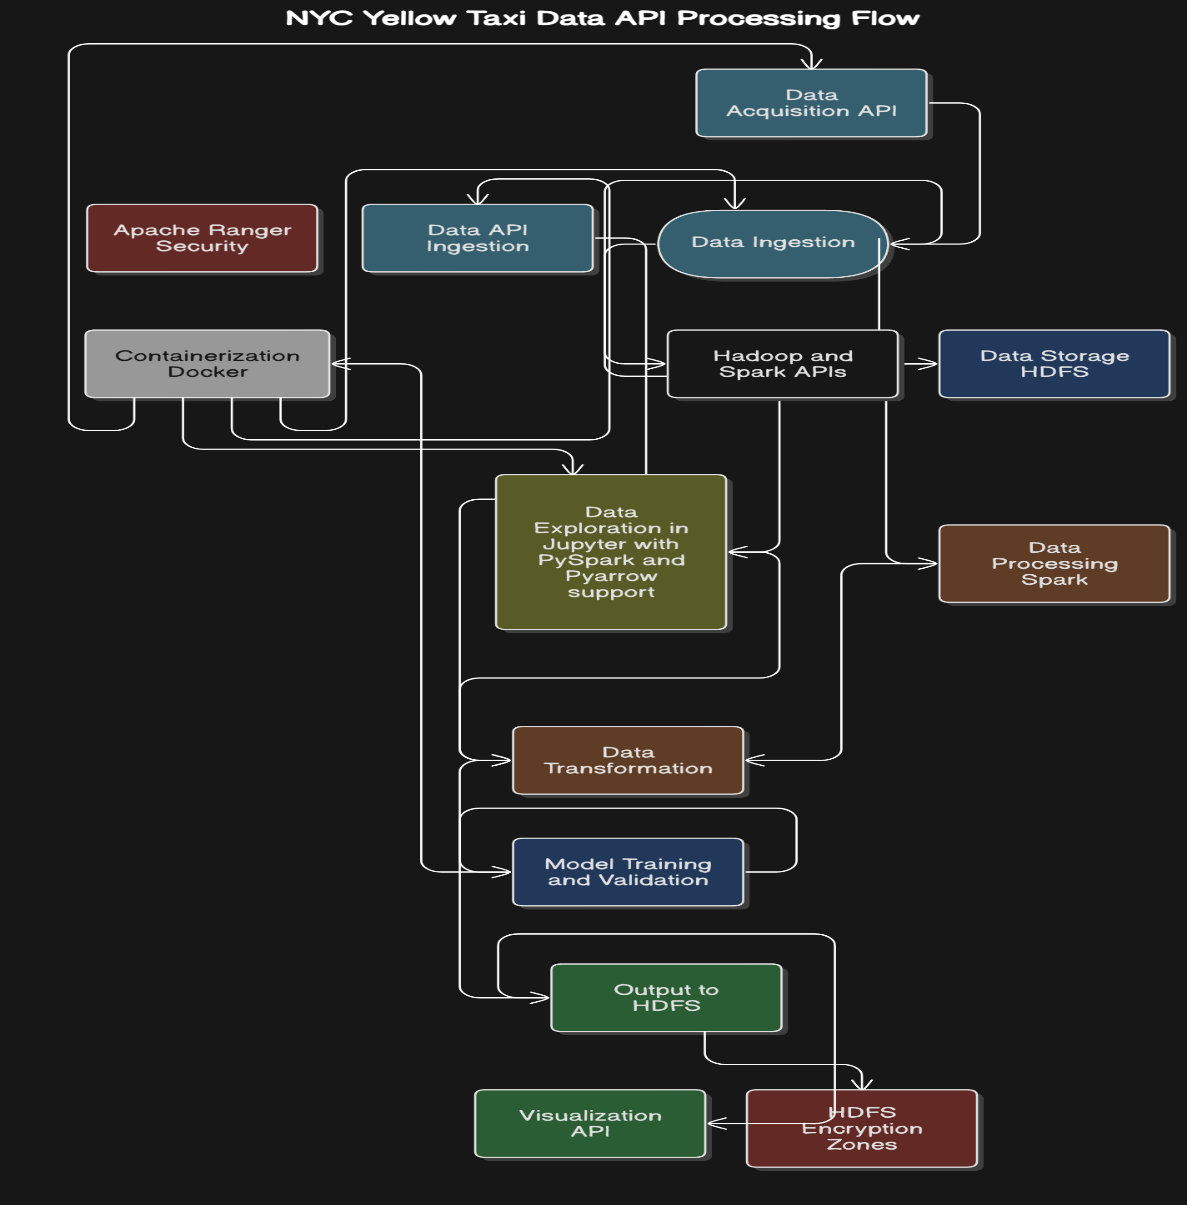
\includegraphics[width=\linewidth]{data-flow-overview.png}
  \centering
  \caption{A high-level overview of the data flow in the tech stack}
\end{figure}

\subsection{Architectural Design}
The proposed system architecture adopts a scalable batch processing pipeline tailored for large-scale data analytics and predictive modeling. It is built upon two core components: the Apache Hadoop Distributed File System (HDFS) for distributed storage, and Apache Spark for high-performance, in-memory batch computation. The primary objective is to process historical trip records from the New York City Taxi and Limousine Commission (NYC TLC) dataset to develop a machine learning model capable of predicting taxi fare amounts.

\subsubsection{Storage Layer – Apache HDFS}
Apache HDFS is employed as the central storage layer within the system. It provides reliable, fault-tolerant distributed storage, enabling efficient access to large volumes of structured and semi-structured data. The following data assets are stored in HDFS:

\begin{itemize}
  \item Raw CSV files obtained from the official NYC TLC trip record dataset.
  \item Cleaned and preprocessed datasets containing filtered and validated trip records.
  \item Feature-engineered training and testing datasets.
  \item Model artifacts, evaluation metrics, and result outputs.
\end{itemize}

HDFS is selected for its scalability and robustness in handling batch-oriented workloads across commodity hardware. Its high-throughput capabilities are particularly well-suited for the sequential read/write patterns common in data science workflows.

\subsubsection{Processing and Modeling Layer – Apache Spark}
Apache Spark serves as the primary computational engine, responsible for executing the full data processing and machine learning pipeline:
\begin{itemize}
  \item Data Preprocessing: Raw taxi trip data is ingested into Spark DataFrames. Data cleansing and transformation steps include filtering invalid records, computing trip duration, and extracting temporal and geospatial features.
  \item Feature Engineering: Additional transformations generate predictive variables such as time-of-day bins and pickup zone clusters.
  \item Model Training: Spark MLlib is utilized to train regression models—such as linear regression and gradient-boosted trees—for fare prediction.
  \item Evaluation and Export: Model performance is assessed using metrics like Root Mean Squared Error (RMSE) and Coefficient of Determination (). Trained models and result datasets are then persisted to HDFS for further analysis or deployment.
\end{itemize}

All processing is conducted in batch mode, leveraging Spark’s distributed in-memory architecture to efficiently handle large-scale datasets.

\subsubsection{Visualization Layer - Jupyter}
The processed data and model outputs are stored in structured formats (e.g., Parquet or CSV) on HDFS. These outputs are then explored and visualized through interactive data science environments such as Jupyter Notebooks using PySpark. Popular Python libraries like matplotlib and seaborn are employed for generating plots, evaluating model predictions, and conducting exploratory data analysis.

\subsection{Resource Allocation}
\begin{itemize}
    \item Budget:
    \begin{itemize}
        \item \$0 for software (open-source stack)
        \item Optional cloud cost if local resources are insufficient
    \end{itemize}
    
    \item \textbf{Hardware Requirements:}
    \begin{itemize}
        \item 1--2 machines (VMs or physical) with:
        \begin{itemize}
            \item 4--8 CPU cores
            \item 8--16 GB RAM
            \item 100--500 GB storage
            \item Docker \& internet access
        \end{itemize}
    \end{itemize}
    
    \item \textbf{Software Stack:}
    \begin{itemize}
        \item Apache Hadoop (HDFS)
        \item Apache Spark
        \item Docker + Docker Compose
        \item Python/Scala (for Spark jobs)
        \item GitHub (for version control)
    \end{itemize}
\end{itemize}

\subsection{Risk Assessment \& Mitigation}

\begin{table}[htbp]
\caption{Risk Assessment and Mitigation Strategies}
\centering
\resizebox{\linewidth}{!}{%
\begin{tabular}{|p{3.8cm}|p{1.8cm}|p{6.4cm}|}
\hline
\textbf{Risk} & \textbf{Impact} & \textbf{Mitigation Strategy} \\
\hline
Inaccurate or incomplete data & High & Apply data validation, drop/filter bad records \\
\hline
Hardware or memory limitations & Medium & Use sampling for tests, scale with cloud/cluster if needed \\
\hline
Docker container issues & Medium & Use Docker Compose, define health checks, log errors \\
\hline
Lack of experience with big data tools & Medium & Share tutorials, divide workload based on familiarity \\
\hline
Coordination difficulty (6-person team) & Medium & Use shared tools (Trello, GitHub, group chat) for collaboration \\
\hline
\end{tabular}%
}
\label{table:risk}
\end{table}

\section{References}
\begin{thebibliography}{15}
\bibitem{tlcdata}
New York City Taxi and Limousine Commission, ``TLC Trip Record Data,'' 2023. [Online]. Available: \url{https://www.nyc.gov/site/tlc/about/tlc-trip-record-data.page}
\bibitem{hdfs}
Apache Hadoop, ``HDFS Architecture Guide,'' 2013. [Online]. Available: \url{https://hadoop.apache.org/docs/r1.2.1/hdfs_design.html}
\bibitem{mllib}
Apache Spark, ``MLlib: Machine Learning Library,'' 2025. [Online]. Available: \url{https://spark.apache.org/mllib/}
\bibitem{matplotlib}
Matplotlib Developers, ``matplotlib.pyplot,'' Matplotlib 3.10.1 Docs. [Online]. Available: \url{https://matplotlib.org/3.5.3/api/_as_gen/matplotlib.pyplot.html}
\bibitem{celerdata}
CelerData, ``Hadoop Distributed File System (HDFS),'' 2024. [Online]. Available: \url{https://celerdata.com/glossary/hadoop-distributed-file-system-hdfs}
\bibitem{hdfspermissions}
Apache Hadoop, ``HDFS Permissions Guide,'' 2022. [Online]. Available: \url{https://hadoop.apache.org/docs/current/hadoop-project-dist/hadoop-hdfs/HdfsPermissionsGuide.html}
\bibitem{ranger}
S. Gattoju and V. Nagalakshmi, ``Design of Apache Ranger framework for securing Hadoop application in big data,'' 2022. [Online]. Available: \url{https://www.researchgate.net/publication/364091563}
\bibitem{ikeorah}
C. Ikeorah, \textit{Optimising Passenger Travel Experience: A Data-Driven Approach Using NYC TLC Trip Record Data}, University of the West of England, 2024. [Online]. Available: \url{https://www.researchgate.net/publication/389370602}
\bibitem{rhouas}
S. Rhouas and N. El Hami, ``Analysis of big data from New York taxi trip 2023: revenue prediction using ordinary least squares solution and limited-memory Broyden-Fletcher-Goldfarb-Shanno algorithms,'' \textit{Int. J. Electr. Comput. Eng. (IJECE)}, vol. 15, no. 1, pp. 711--718, Feb. 2025, doi: 10.11591/ijece.v15i1.pp711-718.
\bibitem{huang}
H. Huang, ``Taxi fare prediction based on multiple machine learning models,'' \textit{Appl. Comput. Eng.}, vol. 16, no. 1, pp. 7--12, Oct. 2023.
\bibitem{zubaid}
Zubaid, ``Predicting New York City Taxi Fares with Supervised Learning,'' Zubaid.co.uk, 2023. [Online]. Available: \url{https://www.zubaid.co.uk/pdf/final-project.pdf}
\bibitem{stoyanovich}
J. Stoyanovich, M. Gilbride, and V. Z. Moffitt, ``Zooming in on NYC Taxi Data with Portal,'' in \textit{Proc. 1st Workshop on Data Science for Social Good (SoGood 2018)}, CEUR Workshop Proc., vol. 2247, pp. 1--6, 2018. [Online]. Available: \url{https://ceur-ws.org/Vol-2247/poster15.pdf}
\bibitem{knime}
KNIME, ``NYC Taxi Visualization: Data Preparation,'' KNIME Hub, 2023. [Online]. Available: \url{https://hub.knime.com/knime/spaces/Examples/50_Applications/49_NYC_Taxi_Visualization/Data_Preparation~yZI74OtdOBVajpsT/current-state}
\bibitem{shylaja}
S. Shylaja and M. K. Nirai Vaani, ``A Machine Learning Framework for Profitability Profiling and Dynamic Price Prediction for the New York City Taxi Trips,'' \textit{Int. J. Innov. Technol. Explor. Eng. (IJITEE)}, vol. 9, no. 5, pp. 973--978, Mar. 2020. [Online]. Available: \url{https://www.ijitee.org/wp-content/uploads/papers/v9i5/E2669039520.pdf}
\end{thebibliography}

\end{document}

